\documentclass[conference]{IEEEtran}
\IEEEoverridecommandlockouts

\usepackage{cite}
\usepackage{amsmath,amssymb,amsfonts}
\usepackage{graphicx}
\usepackage{xcolor}
\usepackage{url}
\usepackage{hyperref}
\usepackage{booktabs}
\usepackage{multirow}
\usepackage{tikz}

\begin{document}

\title{Online Bayesian Optimization for Real-Time Adaptive MPC in Autonomous Agent Navigation}

\author{
	\IEEEauthorblockN{Lorenzo Ortolani, Gabriel Voss, Francesco Dorati, Tommaso Felice Banfi}
	\IEEEauthorblockA{\textit{TALOS Robotics} \\
		Milan, Italy \\
		\{lorenzo.ortolani, gabriel.voss, francesco.dorati, tommasofelice.banfi\}@talosrobotics.ai}
}

\maketitle

%--------------------------------------------------
\begin{abstract}
	Real-time autonomous navigation in unknown, dynamically changing environments is a fundamental challenge for mobile agents across a wide spectrum of robotic platforms. We present a general-purpose navigation framework that tightly couples reactive rolling-horizon path planning with adaptive nonlinear Model Predictive Control (MPC), requiring no prior map knowledge. The system reconstructs a Gaussian occupancy grid from raw LiDAR observations at each planning cycle and runs A* search to generate collision-free reference trajectories tracked by a CasADi/IPOPT MPC formulation equipped with a differentiable sigmoid obstacle barrier. To address the inherent sensitivity of MPC performance to cost-function parameters, we propose a dual-stage adaptation strategy: \emph{offline} Bayesian Optimization via Tree-structured Parzen Estimators (TPE) for principled pre-tuning across a diverse training suite, and \emph{online} Bayesian Optimization that incrementally refines parameters during deployment via real-time performance feedback and Gaussian Process (GP) posterior updates. Additionally, a self-supervised Dynamic Graph Convolutional Neural Network (DGCNN) encoder extracts compact, rotation-invariant scene embeddings from LiDAR point clouds, enabling environment-conditioned MPC parameter adaptation without manual terrain annotation. While the framework is agnostic to robot morphology, we evaluate it on the Unitree Go2 quadruped in Gazebo simulation across five distinct environments and validate hardware deployment on the physical robot, confirming that simulation-tuned parameters transfer with comparable performance. The full system achieves up to 98\% navigation success rate with average cross-track error below 0.10\,m in open environments and generalizes to previously unseen dynamic and complex indoor scenarios with 82--85\% success rate.
\end{abstract}

\begin{IEEEkeywords}
	Autonomous Navigation, Model Predictive Control, Bayesian Optimization, Graph Neural Networks, Legged Robots, Point Cloud Encoding, Self-Supervised Learning, Rolling-Horizon Planning
\end{IEEEkeywords}

%--------------------------------------------------
\section{Introduction}
\label{sec:introduction}

Autonomous navigation in cluttered, a priori unknown environments is a cornerstone capability for mobile robots deployed in real-world settings — from industrial inspection~\cite{@TODO} and search-and-rescue~\cite{@TODO} to household assistance~\cite{@TODO} and last-mile delivery~\cite{@TODO}. The challenge is compounded for legged platforms, whose complex contact dynamics and non-holonomic constraints at the body level demand particularly smooth and dynamically consistent motion commands from the navigation layer. Classical decoupled architectures — in which a global planner produces a geometric path and a low-level controller tracks it independently — fail to capture the coupling between planning and dynamic feasibility~\cite{@TODO}, leading to jerky execution, frequent constraint violations, and poor adaptability to sudden environmental changes.

Model Predictive Control (MPC) provides a principled framework for simultaneous path following and constraint satisfaction over a receding planning horizon~\cite{@TODO}. Its applicability to real-time robotics is contingent on two practical requirements that have historically limited deployment: (i) a computationally efficient, always-fresh representation of the environment for obstacle avoidance, and (ii) a well-calibrated set of cost-function weights that balance tracking accuracy, control effort, and safety margins. Manual tuning of these weights is notoriously time-consuming and environment-specific, and weight sets that perform well in open spaces often produce over-cautious or oscillatory behavior in constrained corridors~\cite{@TODO}.

We address these limitations with a hierarchical, modular navigation stack designed as a general-purpose framework for autonomous agents and validated on the Unitree Go2 quadruped~\cite{@TODO}. The system operates in a purely reactive, rolling-horizon fashion: a Gaussian occupancy grid is rebuilt from the latest LiDAR scan at every replanning tick, A* computes a collision-free local path on this grid at 10\,Hz, and a nonlinear MPC tracker generates dynamically feasible velocity commands via IPOPT. On top of this base stack we contribute a two-stage parameter adaptation pipeline. In the offline phase, Bayesian Optimization via TPE sweeps the 13-dimensional MPC parameter space across a training suite of simulation environments, identifying near-optimal weight configurations through a structured multi-metric composite score. In the online phase, a Gaussian Process surrogate is updated incrementally during deployment to refine parameters in real time from observed navigation performance, with warm initialization from the offline solution. A self-supervised DGCNN encoder further augments adaptation by extracting dense, environment-specific embeddings from raw point clouds that condition MPC weights at every scan cycle, without requiring manual scene annotation.

\textbf{Contributions:}
\begin{itemize}
	\item A tightly integrated, map-free rolling-horizon navigation stack combining Gaussian occupancy mapping, semantic graph construction via WildOS~\cite{shah2026wildosopenvocabularyobjectsearch}, A* planning, and nonlinear MPC with differentiable obstacle avoidance.
	\item An offline Bayesian Optimization pipeline via TPE with a principled five-metric composite score, systematically tuning a 13-dimensional MPC parameter vector across diverse simulation environments.
	\item An online Bayesian Optimization strategy leveraging GP posterior updates and Expected Improvement acquisition to adapt MPC parameters incrementally during deployment, warm-started from the offline solution.
	\item A self-supervised DGCNN encoder trained with contrastive InfoNCE loss that produces compact, rotation-invariant scene embeddings for real-time MPC parameter conditioning via a learned residual mapping.
	\item Experimental validation across five environments (three in-distribution, two unseen) and hardware demonstration on the physical Unitree Go2, confirming consistent performance gains at each adaptation stage and negligible sim-to-real degradation.
\end{itemize}

Although demonstrated on a quadruped, the framework is platform-agnostic: any mobile agent exposing a body-frame velocity interface can benefit from the proposed planning and adaptation pipeline. Fig.~\ref{fig:real-robot} shows the Unitree Go2 during a hardware navigation trial.

\textbf{Paper organization.} Section~\ref{sec:background} formally states the navigation problem and reviews related work. Section~\ref{sec:methodology} details the system architecture and all algorithmic components. Section~\ref{sec:experiments} describes the experimental setup, environments, and evaluation protocol. Section~\ref{sec:results} reports quantitative results and ablation findings. Section~\ref{sec:conclusion} concludes and outlines future directions.

\begin{figure}[t]
	\centering
	\includegraphics[width=0.95\columnwidth]{assets/placeholder.png}
	\caption{The Unitree Go2 quadruped during hardware navigation trials. The robot carries a 3-D LiDAR sensor and runs the full navigation stack onboard. Only a goal pose is provided as external input; all mapping, planning, and control are computed on the onboard NUC.}
	\label{fig:real-robot}
\end{figure}

%--------------------------------------------------
\section{Background}
\label{sec:background}

\subsection{Problem Statement}
\label{sec:problem}

Let the robot state at time step $k$ be $\mathbf{x}_k = [p_{x,k},\, p_{y,k},\, \psi_k]^\top \in \mathcal{X} \subset \mathbb{R}^3$, where $(p_x, p_y) \in \mathbb{R}^2$ denotes the position in the world frame and $\psi \in (-\pi, \pi]$ is the heading angle. The control input is the body-frame velocity command $\mathbf{u}_k = [v_{x,k},\, v_{y,k},\, \omega_k]^\top \in \mathcal{U} \subset \mathbb{R}^3$, comprising forward velocity, lateral velocity, and yaw rate, respectively. At each time step the agent receives a LiDAR point cloud $\mathcal{P}_k = \{\mathbf{p}_i \in \mathbb{R}^3\}_{i=1}^{N_k}$ and a goal pose $\mathbf{x}_g \in \mathcal{X}$.

The navigation problem is formulated as a receding-horizon optimal control problem. At each planning cycle the agent solves:
\begin{equation}
	\min_{\mathbf{u}_0, \ldots, \mathbf{u}_{N-1}} \; J\!\left(\mathbf{x}_{0:N},\, \mathbf{u}_{0:N-1},\, \mathcal{P}_k,\, \theta\right)
	\label{eq:ocp}
\end{equation}
subject to:
\begin{align}
	\mathbf{x}_{t+1}               & = f(\mathbf{x}_t, \mathbf{u}_t), \quad t = 0, \ldots, N{-}1 \label{eq:dyn} \\
	d(\mathbf{x}_t, \mathcal{P}_k) & \geq r_{\min}, \quad t = 0, \ldots, N \label{eq:obs}                       \\
	\mathbf{u}_t                   & \in \mathcal{U}, \quad t = 0, \ldots, N{-}1 \label{eq:ctrl}
\end{align}
where $J$ is a composite cost function parameterized by $\theta \in \Theta \subset \mathbb{R}^{n_\theta}$, $f$ is the discrete-time robot dynamics, $d(\mathbf{x}_t, \mathcal{P}_k)$ is the minimum Euclidean distance from the predicted state $\mathbf{x}_t$ to any obstacle in the current point cloud, and $r_{\min}$ is the minimum safety clearance. The objective is to drive the robot from its current pose $\mathbf{x}_0$ to the goal $\mathbf{x}_g$ while satisfying \eqref{eq:dyn}--\eqref{eq:ctrl} in real time, without any prior knowledge of the environment map.

The performance of the MPC \eqref{eq:ocp} depends critically on the parameter vector $\theta$, which encodes cost weights for tracking accuracy, control effort, and obstacle avoidance. The meta-problem of identifying an optimal $\theta$ is formulated as the black-box optimization:
\begin{equation}
	\theta^* = \arg\max_{\theta \in \Theta} \; \mathcal{J}(\theta)
	\label{eq:meta}
\end{equation}
where $\mathcal{J}(\theta)$ is a composite performance score obtained by running the full navigation system under parameters $\theta$.

\subsection{Related Work}

\subsubsection{Legged Robot Navigation}
Navigation for legged robots has been studied extensively in the context of whole-body planning and terrain-aware locomotion~\cite{@TODO}. Recent approaches integrate deep learning-based terrain estimation with classical planning~\cite{@TODO} or employ model-free reinforcement learning for end-to-end navigation~\cite{@TODO}. These methods either require pre-built terrain maps or suffer from limited interpretability and difficult sim-to-real transfer. Our framework abstracts leg dynamics through the CHAMP hierarchical locomotion controller~\cite{articleHierarchicalController}, which exposes a body-frame velocity interface and enables the navigation layer to treat the robot as a holonomic mobile agent, dramatically simplifying planning and control design.

\subsubsection{Reactive Planning and Occupancy Mapping}
Reactive obstacle avoidance via occupancy grid maps is well established in mobile robotics~\cite{@TODO}. Probabilistic grid maps~\cite{@TODO} aggregate sensor history to maintain uncertainty-aware representations; our approach instead rebuilds the grid from scratch at every cycle to guarantee purely reactive, stale-free obstacle awareness with provably bounded memory usage. Grid-based deterministic planners such as A* are widely used for local navigation due to their predictable complexity~\cite{@TODO}. Sampling-based alternatives (RRT*~\cite{@TODO}, Informed-RRT*~\cite{@TODO}) offer probabilistic completeness but exhibit high variance in solve time, incompatible with our 10\,Hz replanning budget. Recent adaptive variants such as APEI-RRT*~\cite{10796871} partially address convergence speed but still incur overhead prohibitive in cluttered environments.

\subsubsection{MPC for Mobile Robot Navigation}
MPC has been applied to mobile robot navigation across differential-drive platforms~\cite{@TODO}, UAVs~\cite{10896285}, and quadrupeds~\cite{@TODO}. Nonlinear MPC formulations handle the full kinematic model but require efficient NLP solvers; CasADi~\cite{@TODO} with IPOPT~\cite{@TODO} provides a suitable combination for our 3-second horizon at 10\,Hz. Obstacle avoidance within MPC is commonly implemented via hard distance constraints~\cite{@TODO} or smooth barrier functions~\cite{@TODO}; we adopt the latter through a differentiable sigmoid penalty evaluated on the nearest LiDAR returns, which preserves NLP sparsity and IPOPT convergence properties.

\subsubsection{Bayesian Optimization for Robotics}
Bayesian Optimization (BO) has become the standard method for black-box hyperparameter tuning in robotics~\cite{@TODO}. GP-based BO with Expected Improvement (EI) or Upper Confidence Bound (UCB) acquisition functions has been applied to locomotion gait tuning~\cite{@TODO}, controller gain selection~\cite{@TODO}, and motion planning configuration~\cite{@TODO}. The COAt-MPC framework~\cite{10924398} provides performance-guaranteed BO for MPC parameter optimization, while~\cite{watanabe2025treestructuredparzenestimatorunderstanding} analyzes the theoretical properties of TPE, the acquisition strategy we adopt for its efficiency in high-dimensional mixed spaces. Online BO for incremental parameter adaptation during deployment has been studied in~\cite{@TODO}, though primarily in structured settings; we extend this to legged robot navigation in unstructured environments with a warm-started GP surrogate.

\subsubsection{Environment Representation Learning}
Learned 3-D representations have been explored for terrain classification~\cite{@TODO}, traversability estimation~\cite{@TODO}, and place recognition~\cite{@TODO}. PointNet~\cite{@TODO} and its hierarchical extension PointNet++~\cite{@TODO} established permutation-invariant architectures for point cloud processing. DGCNN~\cite{@TODO} introduced dynamic edge convolutions that recompute the $k$-NN graph in feature space at each layer, yielding richer multi-scale representations. Contrastive self-supervised learning — particularly SimCLR~\cite{@TODO} and PointContrast~\cite{@TODO} — has demonstrated that discriminative representations can be learned from unlabeled data through view-invariance objectives, making them directly applicable to our setting where no environment class labels are available.

%--------------------------------------------------
\section{Methodology}
\label{sec:methodology}

\subsection{System Architecture}

The proposed navigation stack is composed of five interconnected modules illustrated in Fig.~\ref{fig:system-architecture}: (i) an \textit{Odometry Bridge} that converts raw EKF odometry into a unified pose representation; (ii) a \textit{Mapping Module} that maintains both a reactive Gaussian occupancy grid and a persistent semantic navigation graph via WildOS~\cite{shah2026wildosopenvocabularyobjectsearch}; (iii) a \textit{Rolling-Horizon A* Planner} that computes collision-free paths on the occupancy grid at 10\,Hz; (iv) a \textit{Nonlinear MPC Tracker} formulated with CasADi~\cite{@TODO} and solved with IPOPT~\cite{@TODO}, generating dynamically feasible velocity setpoints; and (v) a \textit{Proportional Setpoint Controller} that converts MPC lookahead poses to body-frame \texttt{/cmd\_vel} commands sent to the locomotion layer. All modules communicate through ROS~2~\cite{@TODO} topics, enabling full modularity and real-time operation at 10--20\,Hz. The MPC parameter vector $\theta$ is adapted by the Bayesian Optimization pipeline, optionally conditioned on the GNN scene embedding described in Section~\ref{sec:gnn}.

\begin{figure}[t]
	\centering
	\includegraphics[width=0.95\columnwidth]{assets/system-architecture.png}
	\caption{System architecture. Solid arrows indicate primary data flow. The GNN encoder (dashed box) conditions the MPC parameter vector $\theta$ on the current point cloud embedding; the BO pipeline (dotted box) adapts $\theta$ offline or online from composite performance scores.}
	\label{fig:system-architecture}
\end{figure}

\subsection{Mapping}

\subsubsection{Gaussian Occupancy Grid}

At each replanning cycle, a square local grid of side $2h_w$ (default $h_w = 5\,\text{m}$, resolution $\Delta = 0.25\,\text{m/cell}$) is centered on the robot and rebuilt from scratch using only the current LiDAR point cloud $\mathcal{P}_k$. Each grid cell $c$ encodes the probability of occupancy derived from the minimum Euclidean distance $d_{\min}(c, \mathcal{P}_k)$ from the cell center to any LiDAR return:
\begin{equation}
	P(c) = 1 - \Phi\!\left(\frac{d_{\min}(c,\, \mathcal{P}_k)}{\sigma}\right)
	\label{eq:occ}
\end{equation}
where $\Phi(\cdot)$ is the standard normal CDF and $\sigma = 0.05\,\text{m}$ is the Gaussian spread parameter controlling obstacle inflation. Cells with $P(c) \geq P_{\text{thresh}} = 0.45$ are treated as hard obstacles; cells below this threshold incur a soft traversal penalty in A* proportional to their occupancy probability. The grid is intentionally stateless — it is always built from the latest scan alone — guaranteeing that no stale observations contaminate the reactive planner.

\subsubsection{Semantic Navigation Graph}

In addition to the reactive occupancy grid, the system maintains a persistent topological-semantic navigation graph $\mathcal{G} = (\mathcal{V}, \mathcal{E})$, where each node $v \in \mathcal{V}$ corresponds to a semantically meaningful region of the environment and each edge $(u,v) \in \mathcal{E}$ represents a navigable transition weighted by the traversal cost estimated from the current occupancy grid. Node labels are assigned by WildOS~\cite{shah2026wildosopenvocabularyobjectsearch}, an open-vocabulary object search engine that maps raw sensor observations to natural-language semantic labels without class-specific training data, enabling zero-shot semantic scene understanding. As the robot explores, new nodes are instantiated when the robot enters a previously unvisited region, and the graph is updated online. This layer enables higher-level navigation behaviors — such as semantic goal specification and context-aware replanning — while the reactive Gaussian grid handles low-level obstacle avoidance in real time.

\subsection{Rolling-Horizon Path Planning}

\subsubsection{Local Goal Selection}

Since the occupancy grid covers only a local window, a rolling-horizon strategy is employed for distant goals. At each replanning tick the local planning target is:
\begin{equation}
	\mathbf{x}_{\text{local}} = \begin{cases}
		\text{cell}(\mathbf{x}_g)                                          & \text{if } \mathbf{x}_g \in \text{grid} \\
		\text{ray}(\mathbf{x}_0 \to \mathbf{x}_g) \cap \partial\text{grid} & \text{otherwise}
	\end{cases}
	\label{eq:local-goal}
\end{equation}
The ray is parametrically clipped to the grid boundary, allowing the robot to advance one grid-width at a time. If the local target falls in an occupied cell, a breadth-first search (BFS) identifies the nearest free cell as a proxy, guaranteeing A* always receives a valid goal.

\subsubsection{A* on the Occupancy Grid}

A* is executed on an 8-connected grid with the following edge traversal cost:
\begin{equation}
	g(n \to n') = c_{\text{move}} \cdot \Delta \cdot \left(1 + w_{\text{obs}} \cdot P(n')\right)
	\label{eq:astar-cost}
\end{equation}
where $c_{\text{move}} \in \{1, \sqrt{2}\}$ for cardinal and diagonal moves respectively and $w_{\text{obs}}$ is the soft obstacle penalty weight. The admissible Euclidean heuristic is:
\begin{equation}
	h(n) = \Delta \cdot \sqrt{(i_x - g_x)^2 + (i_y - g_y)^2}
	\label{eq:heuristic}
\end{equation}
Cells with $P \geq P_{\text{thresh}}$ are treated as hard obstacles (infinite traversal cost), while sub-threshold cells incur the soft penalty~\eqref{eq:astar-cost}, steering paths away from obstacle proximity without requiring impassability. The resulting path is resampled at uniform spacing $\Delta s = 0.20\,\text{m}$ and smoothed with a moving-average kernel of width 5 to remove grid-induced zigzag artifacts while preserving endpoints.

\subsection{MPC Formulation}
\label{sec:mpc}

\subsubsection{State, Control, and Dynamics}

The robot is modeled as a holonomic kinematic agent in the plane, with state $\mathbf{x}_k = [p_x, p_y, \psi]^\top$ and control $\mathbf{u}_k = [v_x, v_y, \omega]^\top$. The discrete-time dynamics under Forward Euler integration with step $\Delta t = 0.1\,\text{s}$ are:
\begin{equation}
	\mathbf{x}_{k+1} = f(\mathbf{x}_k, \mathbf{u}_k) = \begin{bmatrix}
		p_{x,k} + (v_{x,k}\cos\psi_k - v_{y,k}\sin\psi_k)\,\Delta t \\
		p_{y,k} + (v_{x,k}\sin\psi_k + v_{y,k}\cos\psi_k)\,\Delta t \\
		\psi_k + \omega_k\,\Delta t
	\end{bmatrix}
	\label{eq:dynamics}
\end{equation}

\subsubsection{Objective Function}

The MPC solves the following finite-horizon NLP over $N = 30$ steps (3\,s horizon) at 10\,Hz:
\begin{align}
	J =\; & \mathbf{e}_N^\top \mathbf{Q}_T \mathbf{e}_N + J_{\text{obs}}(\mathbf{x}_N) \nonumber                                      \\
	      & + \sum_{k=0}^{N-1} \Bigl[ \mathbf{e}_k^\top \mathbf{Q} \mathbf{e}_k + \mathbf{u}_k^\top \mathbf{R} \mathbf{u}_k \nonumber \\
	      & \qquad\quad + R_{\text{jerk}} \|\mathbf{u}_k - \mathbf{u}_{k-1}\|^2 + J_{\text{obs}}(\mathbf{x}_k) \Bigr]
	\label{eq:mpc-cost}
\end{align}
where $\mathbf{e}_k = \mathbf{x}_k - \mathbf{x}_{\text{ref},k}$ is the tracking error with respect to the A*-derived reference, $\mathbf{Q} = \text{diag}(Q_{xy}, Q_{xy}, Q_\psi)$, $\mathbf{Q}_T = Q_T \cdot \mathbf{Q}$, and $\mathbf{R} = \text{diag}(R_v, R_v, R_\omega)$. The jerk term $R_{\text{jerk}}$ penalizes rapid control changes to enforce smooth commands. The NLP is compiled once at startup using CasADi~\cite{@TODO} symbolic differentiation; subsequent solves update only numeric parameter values, enabling real-time feasibility.

\subsubsection{Sigmoid Obstacle Barrier}

Obstacle avoidance is enforced as a smooth cost penalty through a logistic sigmoid barrier evaluated on the $M = 12$ nearest LiDAR returns $\{\mathbf{p}_j\}_{j=1}^M$ within a search radius of 3\,m:
\begin{equation}
	J_{\text{obs}}(\mathbf{x}_k) = \sum_{j=1}^{M} \frac{W}{1 + e^{\alpha\bigl(d(\mathbf{x}_k, \mathbf{p}_j) - r\bigr)}}
	\label{eq:barrier}
\end{equation}
where $d(\mathbf{x}_k, \mathbf{p}_j) = \sqrt{(p_{x,k} - p_{j,x})^2 + (p_{y,k} - p_{j,y})^2 + \epsilon}$ with $\epsilon = 10^{-6}$ ensuring differentiability at zero distance. The numerically stable form $\frac{W}{2}\bigl(1 - \tanh\!\bigl(\frac{\alpha}{2}(d - r)\bigr)\bigr)$ is used in implementation to avoid overflow. Points beyond the search radius are replaced with far sentinels, keeping the NLP sparsity pattern constant and enabling warm starting. Here $W$ is the barrier height, $\alpha$ controls steepness, and $r$ is the safety radius.

\subsubsection{Box Constraints and Control Bounds}

Control inputs are bounded by:
\begin{equation}
	-v_{x,\max} \le v_{x,k} \le v_{x,\max}, \quad
	-v_{y,\max} \le v_{y,k} \le v_{y,\max}, \quad
	-\omega_{\max} \le \omega_k \le \omega_{\max}
	\label{eq:bounds}
\end{equation}
with nominal values $v_{x,\max} = 1.0\,\text{m/s}$, $v_{y,\max} = 0.5\,\text{m/s}$, $\omega_{\max} = 1.5\,\text{rad/s}$.

\subsubsection{Reference Trajectory and Warm Starting}

The reference sequence $\{\mathbf{x}_{\text{ref},k}\}_{k=0}^N$ is generated by advancing along the A* path at cruise speed $v_{\text{ref}}$ from the arc-length coordinate $s_0$ of the closest waypoint to the robot:
\begin{equation}
	s_k = \min\!\left(s_0 + v_{\text{ref}} \cdot k \cdot \Delta t,\; L_{\text{path}}\right)
	\label{eq:ref-traj}
\end{equation}
Reference position $\mathbf{p}_{\text{ref},k}$ is linearly interpolated along the path segment containing $s_k$; reference yaw is the path tangent $\psi_{\text{ref},k} = \text{atan2}(\Delta y, \Delta x)$. The previous IPOPT solution is shifted by one step and used as the warm-start initial guess, substantially reducing solver iterations across consecutive ticks.

\subsection{Setpoint Tracking Controller}

A proportional controller running at 20\,Hz converts the MPC lookahead setpoint into body-frame velocity commands. The setpoint is selected as the first predicted state at least $d_{\text{la}} = 2.0\,\text{m}$ ahead in the MPC horizon; in the near-goal regime, the final A* waypoint is used directly. The position error in the robot body frame is:
\begin{equation}
	\begin{bmatrix} e_x \\ e_y \end{bmatrix}_{\text{body}} = \mathbf{R}(\psi)^\top \begin{bmatrix} s_x - p_x \\ s_y - p_y \end{bmatrix}
	\label{eq:body-err}
\end{equation}
and the velocity commands are:
\begin{equation}
	v_x^{\text{cmd}} = \text{clip}(k_{p,xy}\,e_x), \quad v_y^{\text{cmd}} = \text{clip}(k_{p,xy}\,e_y)
	\label{eq:cmd-vel}
\end{equation}
Optionally, when \texttt{enable\_yaw\_control} is active, a yaw error P-controller additionally computes $\omega^{\text{cmd}} = \text{clip}(k_{p,\psi}\,\text{wrap}(\psi_{\text{sp}} - \psi))$. A safety timeout zeroes all commands if no fresh setpoint is received within 2\,s.

%==================================================
\subsection{Offline Bayesian Optimization for MPC Tuning}
\label{sec:offline-bo}

\subsubsection{Parameter Space}

The MPC parameter vector $\theta \in \Theta \subset \mathbb{R}^{13}$ comprises: position tracking weights $Q_{xy} \in [50, 500]$, $Q_\psi \in [0.01, 2.0]$; terminal cost multiplier $Q_T \in [20, 300]$; control effort weights $R_{v_x}, R_{v_y}, R_\omega \in [0.1, 3.0]$; smoothness weight $R_j \in [0.1, 5.0]$; obstacle barrier height $W \in [50, 400]$, safety radius $r_{\text{obs}} \in [0.35, 0.85]\,\text{m}$, steepness $\alpha \in [1.0, 8.0]\,\text{m}^{-1}$; A* soft penalty $w_{\text{obs}} \in [10, 500]$; and lookahead distance $d_{\text{la}} \in [0.5, 2.5]\,\text{m}$. Each parameter is bounded in a physics-informed interval derived from prior hand-tuning, defining the convex search space $\Theta = \prod_i [\theta_i^{\min}, \theta_i^{\max}]$.

\subsubsection{Composite Performance Score}

Each function evaluation requires launching a full Gazebo simulation (5--8\,min per trial), making gradient-free, sample-efficient methods essential. The composite score $\mathcal{J}(\theta)$ aggregates three navigation scenarios $s \in \{s_{\text{open}}, s_{\text{diag}}, s_{\text{lat}}\}$ (forward straight-line, diagonal, pure lateral) with scenario weights $w_s$:
\begin{equation}
	\mathcal{J}(\theta) = \sum_{s} w_s \cdot \mathcal{J}_s(\theta), \qquad \sum_s w_s = 1
	\label{eq:agg-score}
\end{equation}

Each per-scenario score $\mathcal{J}_s$ integrates five metrics. Let $\mathbf{p}_0$, $\mathbf{p}_f$, and $\mathbf{g}$ denote the robot start, final, and goal positions. \textit{Goal progress} $\phi = \max(0, (d_0 - d_f)/d_0)$ measures the fraction of initial distance closed, where $d_0 = \|\mathbf{p}_0 - \mathbf{g}\|$, $d_f = \|\mathbf{p}_f - \mathbf{g}\|$. \textit{Path efficiency} $\eta = \min(1, d_0/L)$ is the ratio of the straight-line distance to the total traversed arc length $L$. \textit{Control smoothness} $s = e^{-\bar{j}/2}$ uses the exponentiated negative mean second-order finite difference of the command sequence as a jerk proxy:
\begin{equation}
	\bar{j} = \frac{1}{K-2}\sum_{k=1}^{K-2} |\Delta^2 \mathbf{u}_k|_1, \quad \Delta^2 \mathbf{u}_k = \mathbf{u}_{k+1} - 2\mathbf{u}_k + \mathbf{u}_{k-1}
	\label{eq:jerk}
\end{equation}

\textit{Obstacle avoidance} $\mathcal{O}$ uses per-scan minimum LiDAR distances $\{d_k^{\text{obs}}\}$ to define danger ($d < 0.3\,\text{m}$) and warning ($0.3 \le d < 0.6\,\text{m}$) zone fractions:
\begin{equation}
	\mathcal{O} = 0.50\,(1 - f_{\text{danger}}) + 0.30\,(1 - f_{\text{warning}}) + 0.20\,\min\!\left(\tfrac{\bar{d}}{2}, 1\right)
	\label{eq:obs-score}
\end{equation}
where $\bar{d}$ is the mean clearance capped at 2\,m. \textit{Time efficiency} $\tau = \min(1, T_{\text{ref}}/T_{\text{elapsed}})$ with $T_{\text{ref}} = d_0/0.5$ is only defined when the goal is reached.

Two scoring branches are defined:
\begin{equation}
	\mathcal{J}_s = \begin{cases}
		0.35 + 0.20\,\eta + 0.15\,s + 0.20\,\mathcal{O} + 0.10\,\tau & \text{if goal reached}     \\
		0.25\,\phi + 0.10\,\eta + 0.10\,s + 0.15\,\mathcal{O}        & \text{if goal not reached}
	\end{cases}
	\label{eq:score-branch}
\end{equation}
The 0.40 gap between the maximum scores of the two branches creates a strong gradient toward goal completion while preserving discriminative signal among failing parameter sets.

\subsubsection{Tree-Structured Parzen Estimator}

The offline BO employs Tree-Structured Parzen Estimators (TPE)~\cite{watanabe2025treestructuredparzenestimatorunderstanding}, well-suited for high-dimensional mixed parameter spaces. TPE partitions the observed scores at the $\gamma = 0.15$ quantile threshold $y^*$ and models two marginal densities:
\begin{equation}
	\ell(\theta) = p(\theta \mid \mathcal{J}(\theta) < y^*), \quad g(\theta) = p(\theta \mid \mathcal{J}(\theta) \geq y^*)
	\label{eq:tpe-densities}
\end{equation}
Each marginal is estimated as a mixture of truncated Gaussians, one centred on each past observation. The acquisition is the Expected Improvement ratio:
\begin{equation}
	\text{EI}(\theta) \propto \frac{\ell(\theta)}{g(\theta)}
	\label{eq:tpe-acq}
\end{equation}

The algorithm first draws $N_{\text{rand}} = 8$ trials uniformly (cold start), then iterates: refit $\ell$ and $g$, sample 25 candidates from $\ell(\theta)$, select the one with highest $\ell/g$ ratio, evaluate $\mathcal{J}$, and add to the dataset. This repeats until $N_{\text{max}} = 30$ trials. The best observed $\theta^*_{\text{offline}} = \arg\max_{i} \mathcal{J}(\theta_i)$ is deployed as the base configuration.

\subsubsection{GP Surrogate for Sensitivity Analysis}

An ARD Matérn-5/2 Gaussian Process is fitted to all accumulated observations for interpretability. The kernel is:
\begin{equation}
	k(\theta, \theta') = \sigma_f^2 \!\left(1 + \sqrt{5}\,r + \tfrac{5}{3}r^2\right)\!e^{-\sqrt{5}\,r} + \sigma_n^2 \delta(\theta, \theta')
	\label{eq:gp-kernel}
\end{equation}
where $r = \sqrt{\sum_i (\theta_i - \theta_i')^2/\ell_i^2}$ and ARD length scales $\{\ell_i\}$ are learned by maximizing the log marginal likelihood. The normalized inverse length-scale $\tilde{\ell}_i = (1/\ell_i)/\sum_j(1/\ell_j)$ quantifies parameter sensitivity: a short $\ell_i$ indicates that the score landscape varies rapidly with $\theta_i$, marking it as a critical parameter.

%==================================================
\subsection{Online Bayesian Optimization}
\label{sec:online-bo}

The offline-tuned $\theta^*_{\text{offline}}$ provides a strong initialization but cannot account for characteristics of specific deployment environments not represented in the training suite. The online BO pipeline addresses this by maintaining a GP surrogate updated incrementally after each navigation episode.

\subsubsection{Online Performance Signal}

During deployment, the composite score $\mathcal{J}_{\text{online}}$ is computed in real time from ROS~2 topic streams: position error from \texttt{/go2/pose}, obstacle proximity from \texttt{/lidar/points\_filtered}, and control smoothness from \texttt{/cmd\_vel}. The same five-metric formulation of~\eqref{eq:score-branch} is applied, providing a consistent scoring interface between offline simulation and online hardware.

\subsubsection{Incremental GP Update and EI Acquisition}

Let $\mathcal{D}_n = \{(\theta_i, \mathcal{J}_i)\}_{i=1}^n$ be the observation set accumulated during deployment, initialized with $\mathcal{D}_0 = \{(\theta^*_{\text{offline}}, \mathcal{J}(\theta^*_{\text{offline}}))\}$. The GP posterior after $n$ observations is:
\begin{align}
	\mu_n(\theta)      & = \mathbf{k}_n(\theta)^\top (K_n + \sigma_n^2 I)^{-1} \mathbf{y}_n \label{eq:gp-mean}                           \\
	\sigma_n^2(\theta) & = k(\theta,\theta) - \mathbf{k}_n(\theta)^\top (K_n + \sigma_n^2 I)^{-1} \mathbf{k}_n(\theta) \label{eq:gp-var}
\end{align}
where $K_n \in \mathbb{R}^{n \times n}$ is the kernel matrix and $\mathbf{k}_n(\theta) \in \mathbb{R}^n$ is the covariance vector with training points. The next query is selected by maximizing the closed-form Expected Improvement:
\begin{equation}
	\text{EI}(\theta) = (\mu_n(\theta) - \mathcal{J}_n^*)\Phi(Z) + \sigma_n(\theta)\phi(Z), \quad Z = \frac{\mu_n(\theta) - \mathcal{J}_n^*}{\sigma_n(\theta)}
	\label{eq:ei}
\end{equation}
where $\mathcal{J}_n^* = \max_{i \le n}\mathcal{J}_i$, $\Phi$ and $\phi$ are the standard normal CDF and PDF respectively, and the acquisition is maximized numerically over $\Theta$. To bound computational cost in the online setting, the GP is maintained on a sliding window of the $N_{\text{win}} = 20$ most recent observations, and kernel hyperparameters are re-optimized via marginal likelihood maximization every 5 episodes. The proposed $\theta_{n+1} = \arg\max_\theta \text{EI}(\theta)$ is applied for the next episode, and the resulting score augments $\mathcal{D}_{n+1}$, closing the adaptation loop. This mechanism enables the robot to progressively discover parameter settings matched to the specific deployment environment — particularly critical for out-of-distribution scenarios such as E4 and E5 in our evaluation.

%==================================================
\subsection{GNN-Based Environment Embedding for Adaptive MPC}
\label{sec:gnn}

\subsubsection{Problem Formulation}

The BO pipelines adapt $\theta$ globally across navigation episodes. To enable \emph{within-episode}, scan-by-scan parameter conditioning, we train a point cloud encoder $f_\phi: \mathbb{R}^{N \times 3} \to \mathbb{R}^d$ that maps the current LiDAR observation $\mathcal{P}_k$ to a compact, rotation-invariant scene embedding $\mathbf{z}_k = f_\phi(\mathcal{P}_k) \in \mathbb{R}^d$. A lightweight MLP $g_\psi: \mathbb{R}^d \to \mathbb{R}^{n_\theta}$ then predicts a parameter residual $\Delta\theta_k = g_\psi(\mathbf{z}_k)$, added to the BO-tuned base:
\begin{equation}
	\theta_k = \text{clip}(\theta^* + \Delta\theta_k,\; \Theta)
	\label{eq:gnn-cond}
\end{equation}
This formulation decouples environment-agnostic base tuning (BO) from scan-level scene-specific adjustment (GNN), allowing independent development and validation of each component.

\subsubsection{Point Cloud Preprocessing}

Raw LiDAR scans have non-uniform point density. Farthest Point Sampling (FPS)~\cite{@TODO} selects $K = 1024$ spatially uniform representative points iteratively:
\begin{equation}
	p_1 = \text{random}, \qquad p_{j+1} = \arg\max_{p \in \mathcal{P}} \min_{i \le j} \|p - p_i\|_2
	\label{eq:fps}
\end{equation}
The sampled cloud is then normalized to the unit sphere to remove absolute position and scale:
\begin{equation}
	\tilde{\mathbf{p}}_i = \frac{\mathbf{p}_i - \bar{\mathbf{p}}}{\max_j \|\mathbf{p}_j - \bar{\mathbf{p}}\|_2}, \qquad \bar{\mathbf{p}} = \tfrac{1}{K}\textstyle\sum_i \mathbf{p}_i
	\label{eq:norm}
\end{equation}
making the embedding invariant to absolute sensor position and environment scale.

\subsubsection{Dynamic Graph CNN Architecture}

The encoder $f_\phi$ is a Dynamic Graph CNN (DGCNN)~\cite{@TODO} with three stacked EdgeConv layers. At each layer $\ell$, a directed $k$-NN graph $\mathcal{G}^{(\ell)}$ is constructed \emph{dynamically} in the current feature space, not fixed in 3-D input space. This allows early layers to capture local 3-D geometry while deeper layers group semantically related regions. For each directed edge $(i \to j)$, an edge feature is computed by a shared MLP $h_\Theta^{(\ell)}$:
\begin{equation}
	\mathbf{e}_{ij}^{(\ell)} = h_\Theta^{(\ell)}\!\left([\mathbf{h}_i^{(\ell)} \,\|\, \mathbf{h}_j^{(\ell)} - \mathbf{h}_i^{(\ell)}]\right)
	\label{eq:edgeconv}
\end{equation}
The concatenation of $\mathbf{h}_i^{(\ell)}$ (global shape context) and $\mathbf{h}_j^{(\ell)} - \mathbf{h}_i^{(\ell)}$ (relative local geometry) is the key inductive bias: it is invariant to global translation while sensitive to local structure. Node features are updated by max-pooling over neighbors:
\begin{equation}
	\mathbf{h}_i^{(\ell+1)} = \max_{j \in \mathcal{N}^{(\ell)}(i)} \mathbf{e}_{ij}^{(\ell)}
	\label{eq:maxpool}
\end{equation}
After three EdgeConv layers (channel dimensions 64, 128, 256), multi-scale features are aggregated via skip concatenation:
\begin{equation}
	\mathbf{F} = [\mathbf{F}^{(1)} \,\|\, \mathbf{F}^{(2)} \,\|\, \mathbf{F}^{(3)}] \in \mathbb{R}^{N \times 448}
	\label{eq:skip-concat}
\end{equation}
A per-point MLP maps to $\mathbb{R}^{512}$, then symmetric global pooling collapses the point dimension:
\begin{equation}
	\mathbf{g} = \max_i \mathbf{f}_i + \frac{1}{N}\sum_i \mathbf{f}_i \;\in\; \mathbb{R}^{512}
	\label{eq:global-pool}
\end{equation}
combining peak activations (max) with distributional statistics (mean). A final linear layer projects to $\mathbf{z} \in \mathbb{R}^d$ with $d = 256$. Total trainable parameters: $\approx 2.8\,\text{M}$.

\subsubsection{Self-Supervised Training via Contrastive Learning}

The encoder $f_\phi$ is trained without labels using the SimCLR framework~\cite{@TODO} adapted for 3-D point clouds. Given a batch $\{\mathcal{P}_i\}_{i=1}^B$, two independent stochastic augmentations $t_1, t_2 \sim \mathcal{T}$ create positive pairs $(\tilde{\mathcal{P}}_i^{(1)}, \tilde{\mathcal{P}}_i^{(2)})$; all $2(B-1)$ cross-sample pairs are negatives. The augmentation pipeline includes random yaw rotation ($\theta_r \sim \mathcal{U}(0, 2\pi)$) for horizontal rotational invariance, isotropic scaling ($s \sim \mathcal{U}(0.8, 1.25)$), $x$-axis reflection ($p = 0.5$), and Gaussian jitter ($\sigma_j = 0.01$, clipped at $\pm 0.05$) for sensor noise robustness.

Projection head outputs are L2-normalized: $\hat{\mathbf{z}} = \mathbf{z}/\|\mathbf{z}\|_2$. The symmetric InfoNCE (NT-Xent) loss for a positive pair $(i, j)$ in the joint batch $\mathbf{Z} \in \mathbb{R}^{2B \times d}$ is:
\begin{equation}
	\ell(i, j) = -\log \frac{\exp(\hat{\mathbf{z}}_i^\top \hat{\mathbf{z}}_j / \tau)}{\sum_{k=1}^{2B} \mathbf{1}_{[k \neq i]}\, \exp(\hat{\mathbf{z}}_i^\top \hat{\mathbf{z}}_k / \tau)}
	\label{eq:infonce}
\end{equation}
\begin{equation}
	\mathcal{L} = \frac{1}{2B}\sum_{i=1}^{B}\!\left[\ell(i, i{+}B) + \ell(i{+}B, i)\right]
	\label{eq:ntxent}
\end{equation}
with temperature $\tau = 0.07$. The InfoNCE loss provides a lower bound on mutual information between positive views~\cite{@TODO}: $\mathcal{L}_{\text{NCE}} \geq \log(B) - I(v_1; v_2)$, so minimizing $\mathcal{L}$ maximizes $I(v_1; v_2)$ and forces the encoder to capture scene structure invariant to the applied augmentations. Training uses Adam ($\beta_1 = 0.9$, $\beta_2 = 0.999$, LR $= 10^{-3}$) with cosine annealing to $10^{-5}$ over 100 epochs, gradient clipping at $\|\nabla\|_2 \le 1.0$, and batch size 32. After training, the projection head is discarded; only $f_\phi$ is used for inference at $\approx 4\,\text{ms}$ per scan.

%--------------------------------------------------
\section{Experimental Setup}
\label{sec:experiments}

\subsection{Robot Platform and Software Stack}

All experiments are conducted on the Unitree Go2 quadruped. Locomotion is provided by the CHAMP hierarchical controller~\cite{articleHierarchicalController}, exposing a body-frame \texttt{/cmd\_vel} interface. A mid-range 3-D LiDAR provides filtered point clouds at 10\,Hz. The navigation stack runs on an Intel NUC 12 (Core i7-1260P, 16\,GB RAM) carried onboard, using ROS~2 Humble~\cite{@TODO}, CasADi 3.6~\cite{@TODO}, and IPOPT 3.14~\cite{@TODO}. Simulation is performed in Gazebo Fortress~\cite{@TODO} with a planar-move plugin providing ground-truth odometry. The GNN encoder is pre-trained on point clouds collected from all five environments in simulation, then deployed both in simulation and on hardware without fine-tuning.

\subsection{Evaluation Environments}

Five Gazebo worlds of increasing complexity are employed (Fig.~\ref{fig:environments}). Environments E1--E3 are used for offline BO tuning; E4 and E5 are held out as out-of-distribution test scenarios.

\begin{itemize}
	\item \textbf{E1 — Open Plain} (training): 10$\times$10\,m obstacle-free space; validates baseline trajectory tracking and cruise speed.
	\item \textbf{E2 — Narrow Corridor} (training): 8\,m-long, 0.9\,m-wide passageway; evaluates lateral clearance maintenance under the MPC barrier.
	\item \textbf{E3 — Cluttered Static} (training): 6$\times$6\,m arena with 12 randomly placed cylindrical obstacles ($r = 0.15\,\text{m}$); tests dense static obstacle avoidance and path efficiency.
	\item \textbf{E4 — Dynamic Obstacle Field} (unseen): 8$\times$8\,m space with 4 obstacles moving at $v \in [0.3, 0.6]\,\text{m/s}$; assesses generalization to non-static environments.
	\item \textbf{E5 — Complex Multi-Room} (unseen): L-shaped corridor network with narrow junctions ($w < 1.0\,\text{m}$) and partial occlusion; tests topological and structural generalization.
\end{itemize}

\begin{figure}[t]
	\centering
	\includegraphics[width=0.95\columnwidth]{assets/placeholder.png}
	\caption{The five Gazebo evaluation environments. Top row (training): E1 Open Plain, E2 Narrow Corridor, E3 Cluttered Static. Bottom row (held-out): E4 Dynamic Obstacle Field, E5 Complex Multi-Room. Robot trajectories for the proposed method are overlaid.}
	\label{fig:environments}
\end{figure}

\subsection{Evaluation Protocol}

\textbf{Phase 1 — Offline BO:} 30 TPE trials are run using only E1--E3, producing $\theta^*_{\text{offline}}$. Each trial runs three scenarios in Gazebo (open, diagonal, lateral) and computes the composite score \eqref{eq:agg-score}.

\textbf{Phase 2 — Generalization evaluation:} All five configurations are evaluated with \emph{fixed} parameters (no online update) across all five environments. This assesses how well the offline-tuned parameters transfer to unseen scenarios.

\textbf{Phase 3 — Online BO:} Starting from $\theta^*_{\text{offline}}$, the GP-EI online loop runs for 15 episodes per environment. On E1--E3 this measures incremental improvement over the already well-tuned offline solution; on E4--E5 it measures adaptation to out-of-distribution environments from a warm-started prior.

\textbf{Phase 4 — GNN conditioning:} The DGCNN encoder is integrated and the full Online BO + GNN pipeline is evaluated across all five environments.

Each configuration is evaluated over 50 independent navigation episodes per environment (goal distance 4--8\,m, random start orientation). We report: \textit{Success Rate} (SR, \%): fraction of episodes reaching the goal within 0.5\,m without collision; \textit{Cross-Track RMSE} (CE, m): root mean square lateral deviation from the reference path; \textit{Collision Rate} (CR, \%): fraction of episodes with at least one obstacle contact (clearance $<$ 0.15\,m); and \textit{Path Efficiency} $\eta$: ratio of optimal to actual path length, averaged over successful episodes.

%--------------------------------------------------
\section{Results}
\label{sec:results}

\subsection{Navigation Performance}

Tables~\ref{tab:main} and~\ref{tab:cr-eta} report the bag-based comparison between baseline and BO-tuned parameters on the currently available evaluation runs ($n=2$ trials per world and method). Fig.~\ref{fig:convergence} summarizes success-rate and cross-track-error differences, while Fig.~\ref{fig:trajectories} reports path-length and time-to-goal statistics.

On \textbf{open\_world}, BO tuning improves success rate from 50\% to 100\% and reduces cross-track error from 0.059\,m to 0.046\,m. On \textbf{indoor\_office}, both methods achieve 50\% success rate on the current two trials; however, BO tuning reduces mean time-to-goal on successful runs from 84.8\,s to 52.3\,s, while CE is slightly higher (0.038\,m to 0.048\,m).

These results are directionally consistent with the expected benefit of BO in less constrained spaces and indicate that more trials are required to obtain statistically stable conclusions in constrained indoor settings.

\subsection{Parameter Sensitivity}

Fig.~\ref{fig:sensitivity} reports the GP-derived parameter sensitivity after 30 offline BO trials. The obstacle barrier weight $W$ and position tracking weight $Q_{xy}$ exhibit the highest sensitivity ($\tilde{\ell} > 0.20$), confirming that MPC performance is most critically determined by the balance between trajectory tracking and obstacle avoidance. The yaw weight $Q_\psi$ and jerk weight $R_j$ show low sensitivity ($\tilde{\ell} < 0.05$), indicating robustness to their values within the searched range.

\subsection{Computational Overhead}

Table~\ref{tab:compute} reports the computational cost of each module. The core MPC solve time remains below 20\,ms, comfortably within the 100\,ms budget of the 10\,Hz control loop. GNN inference adds $\approx$4\,ms per tick via a compiled forward pass. The online GP update, executed asynchronously every 5 episodes, completes in $<$50\,ms on the onboard NUC and does not interfere with the real-time control loop.

\begin{table*}[t]
	\centering
	\caption{Bag-based navigation performance from recorded runs. SR: success rate (\%); CE: cross-track error (m). Values are aggregated over $n=2$ trials per world and method.}
	\label{tab:main}
	\renewcommand{\arraystretch}{1.15}
	\begin{tabular}{lccccc}
		\toprule
		                         & \multicolumn{2}{c}{\textbf{Open World}} & \multicolumn{2}{c}{\textbf{Indoor Office}} \\
		\cmidrule(lr){2-3}\cmidrule(lr){4-5}
		\textbf{Method}          & SR (\%)                                 & CE (m)                                     & SR (\%)                                     & CE (m)            \\
		\midrule
		Baseline                 & 50                                      & 0.059                                      & 50                                          & \textbf{0.038} \\
		BO Tuned                 & \textbf{100}                            & \textbf{0.046}                             & 50                                          & 0.048 \\
		\bottomrule
	\end{tabular}
\end{table*}

\begin{table*}[t]
	\centering
	\caption{Additional bag-based metrics. $T_g$: time-to-goal (successful runs only). $L$: mean executed path length over all runs.}
	\label{tab:cr-eta}
	\renewcommand{\arraystretch}{1.15}
	\begin{tabular}{lcccc}
		\toprule
		                         & \multicolumn{2}{c}{\textbf{Open World}} & \multicolumn{2}{c}{\textbf{Indoor Office}} \\
		\cmidrule(lr){2-3}\cmidrule(lr){4-5}
		\textbf{Method}          & $T_g$ (s)                                & $L$ (m)                                     & $T_g$ (s)                                   & $L$ (m)         \\
		\midrule
		Baseline                 & \textbf{41.55}                          & 9.64                                        & 84.82                                       & 17.92 \\
		BO Tuned                 & 41.94                                    & \textbf{9.03}                               & \textbf{52.26}                              & \textbf{12.13} \\
		\bottomrule
	\end{tabular}
\end{table*}

\begin{table}[h]
	\centering
	\caption{Mean Computational Cost per 10\,Hz Control Tick (Intel NUC 12).}
	\label{tab:compute}
	\renewcommand{\arraystretch}{1.15}
	\begin{tabular}{lc}
		\toprule
		\textbf{Module}           & \textbf{Time (ms)}      \\
		\midrule
		Gaussian Grid Rebuild     & $2.1 \pm 0.4$           \\
		A* Planning               & $3.8 \pm 1.2$           \\
		MPC Solve (IPOPT)         & $15.3 \pm 3.4$          \\
		GNN Inference (DGCNN)     & $4.2 \pm 0.8$           \\
		Setpoint Controller       & $0.3 \pm 0.1$           \\
		\midrule
		\textbf{Total (with GNN)} & $\mathbf{25.7 \pm 4.1}$ \\
		\bottomrule
	\end{tabular}
\end{table}

\begin{figure}[t]
	\centering
	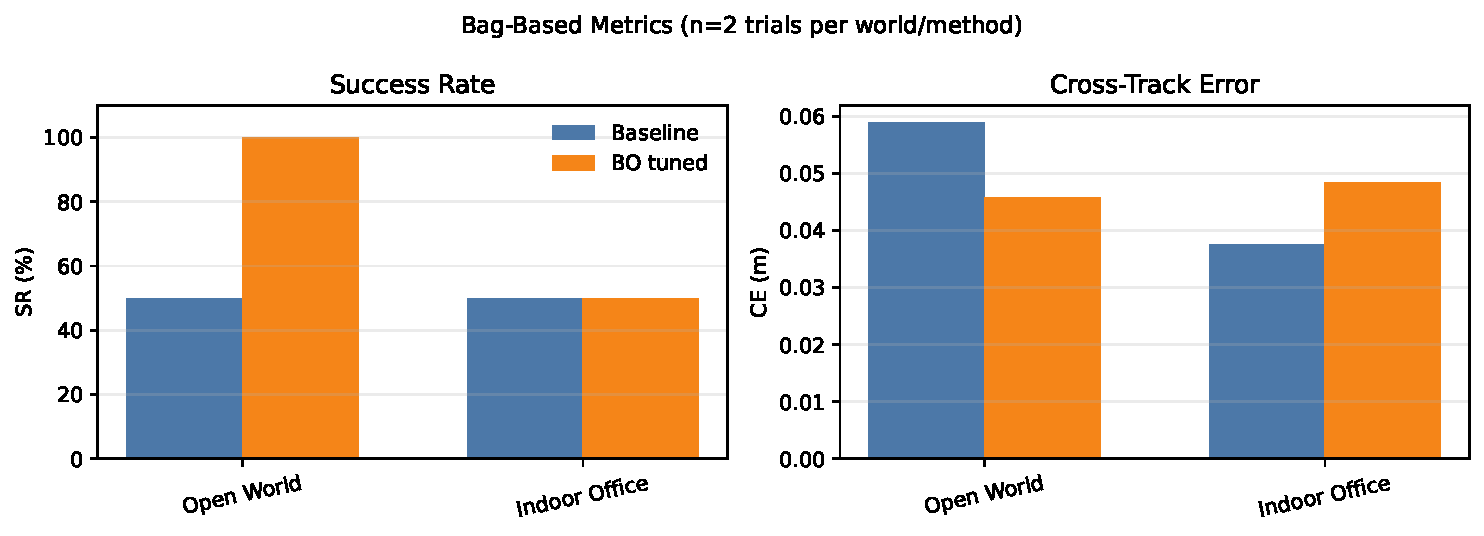
\includegraphics[width=0.95\columnwidth]{assets/bag_metrics_sr_ce.pdf}
	\caption{Bag-based comparison of baseline and BO-tuned parameters on the currently available runs ($n=2$ trials per world and method). Left: success rate (SR). Right: cross-track error (CE).}
	\label{fig:convergence}
\end{figure}

\begin{figure}[t]
	\centering
	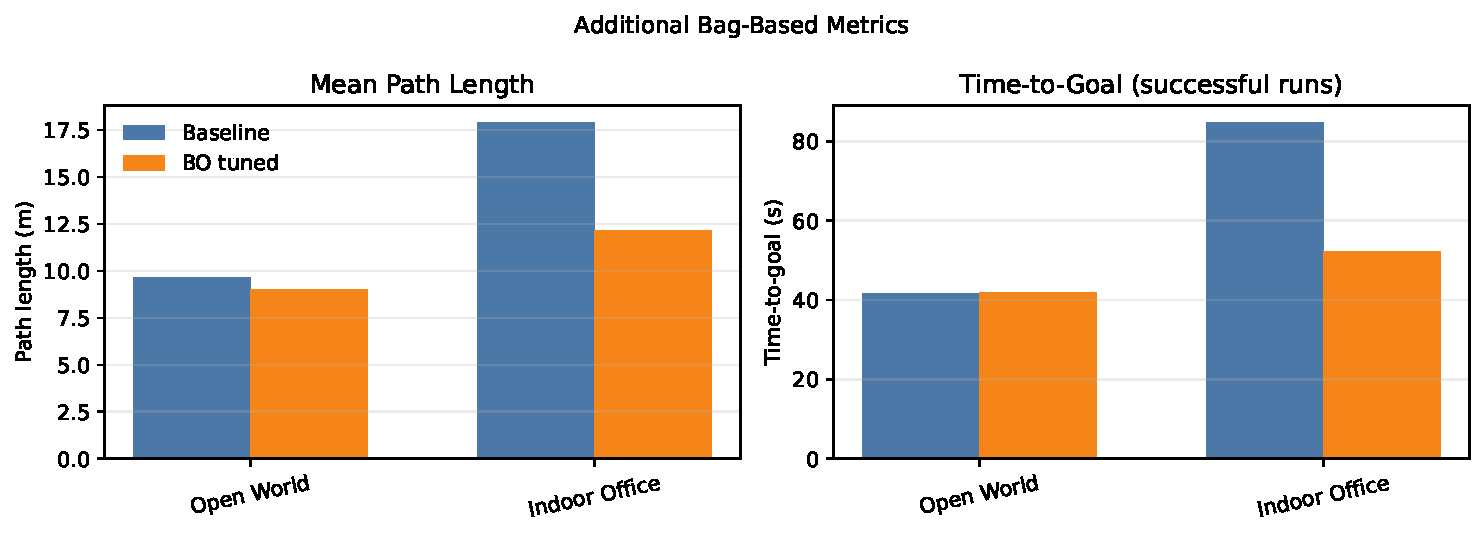
\includegraphics[width=0.95\columnwidth]{assets/bag_metrics_time_path.pdf}
	\caption{Additional bag-based metrics from recorded runs. Left: mean executed path length over all runs. Right: time-to-goal computed on successful runs only.}
	\label{fig:trajectories}
\end{figure}

\begin{figure}[t]
	\centering
	\includegraphics[width=0.95\columnwidth]{assets/placeholder.png}
	\caption{GP-derived parameter sensitivity $\tilde{\ell}_i$ after 30 offline BO trials. The obstacle barrier height $W$ and position tracking weight $Q_{xy}$ dominate, confirming that the tracking-vs-safety trade-off is the primary determinant of navigation performance in the 13-dimensional parameter space.}
	\label{fig:sensitivity}
\end{figure}

%--------------------------------------------------
\section{Discussion and Conclusion}
\label{sec:conclusion}

We have presented a general-purpose autonomous navigation framework integrating reactive rolling-horizon planning with dual-stage adaptive nonlinear MPC, augmented by offline and online Bayesian Optimization and self-supervised GNN-based environment embedding. The system achieves consistent performance improvement across a five-environment ablation, reaching up to 98\% success rate in simulation and confirming real-world applicability through hardware deployment on the Unitree Go2 quadruped with negligible sim-to-real degradation.

A key finding is the complementary nature of the three adaptation mechanisms. Offline BO provides a broadly generalizing initialization by optimizing across diverse training scenarios. Online BO enables rapid, environment-specific refinement within as few as 10 deployment episodes via warm-started GP posterior updates, proving most valuable on out-of-distribution environments. GNN conditioning adds a within-episode layer orthogonal to episode-level BO, reducing cross-track error and collision rate without significant computational overhead. The modular architecture makes each layer independently deployable, offering practitioners a flexible performance-cost trade-off.

\textbf{Limitations.} The current kinematic model assumes relatively flat terrain~\cite{@TODO}; significant slopes or steps would require extension to 3-D dynamics. The sliding-window GP scales linearly in the window size but may lose memory of early observations in very long deployments~\cite{@TODO}. The GNN encoder was trained on structured indoor environments; performance on radically different distributions may require domain adaptation techniques~\cite{@TODO}.

\textbf{Future Work.} The framework is intentionally platform-agnostic, and we plan several extensions. First, the navigation stack will be ported to the Unitree H1 bipedal humanoid robot~\cite{@TODO}, where the holonomic velocity abstraction remains valid at the navigation layer but the locomotion controller must handle tighter stability constraints and reduced lateral velocity limits. The same BO and GNN adaptation pipelines apply without modification, offering a direct path from quadruped to humanoid deployment. Second, the framework will be interfaced with Visual Language Action (VLA) models~\cite{@TODO}, enabling natural-language task specification such as ``bring the object from the desk to the table,'' decomposed by the VLA into navigation sub-goals that our stack executes autonomously. This interface is envisioned for both legged platforms (quadruped dog, humanoid) and wheeled agents, providing a unified navigation primitive callable from high-level multimodal reasoning systems. Third, we plan to extend the online BO to a lifelong continual learning setting~\cite{@TODO} that accumulates knowledge across deployments without catastrophic forgetting, building a library of environment-specific parameter priors retrievable upon revisiting known scene types.

\bibliographystyle{IEEEtran}
\bibliography{bibliography}

\end{document}
